\documentclass[12pt]{article}

% Base packages
\usepackage[round]{natbib}
\usepackage[T1]{fontenc}
\usepackage[utf8]{inputenc}
\usepackage{algorithm}
\usepackage{algpseudocode}
\usepackage{amsfonts}
\usepackage{amsmath}
\usepackage{amssymb}
\usepackage{array}
\usepackage{booktabs}
\usepackage{caption}
\usepackage{enumitem}
\usepackage{fancyhdr}
\usepackage{geometry}
\usepackage{graphicx}
\usepackage{hyperref}
\usepackage{listings}
\usepackage{multirow}
\usepackage{pdfpages}
\usepackage{subcaption}
\usepackage{tikz}
\usepackage{xcolor}

% To ensure citations are a single hyperlink
\makeatletter
\renewcommand\hyper@natlinkbreak[2]{#1}
\makeatother


\title{Report on \textit{Attention Is All You Need}\\\vspace{0.5cm}\large Submitted in Partial Fulfillment of the Requirements for Seminars During the Hilary Term}
\author{Ion Lipsiuc}
\date{\today}

\begin{document}

\maketitle

\begin{abstract}\noindent This report provides an in-depth analysis of the influential paper \textit{Attention Is All You Need},\footnote{See \citep{vaswani2017attention}.} which introduces the transformer model - a groundbreaking architecture that relies entirely on attention mechanisms, thereby eliminating the need for recurrence. We detail the model's core components, including self-attention, multi-head attention, and positional encodings, and review experimental results that demonstrate its significant performance improvements on machine translation tasks.\end{abstract}

\tableofcontents
\newpage

\section{Introduction}

Recent advances in natural language processing (NLP) have been driven by the need to improve the way models handle sequential data, especially in tasks such as machine translation. Traditionally, recurrent neural networks (RNNs) and their variants, although effective, have encountered limitations in capturing long-range dependencies due to their sequential processing nature. These limitations have motivated researchers to explore more parallelizable and efficient approaches.

In their seminal work, \textit{Attention Is All You Need}, the authors introduce the transformer - a novel architecture that completely abandons recurrence in favour of a self-attention mechanism. Unlike RNN-based models, the transformer is capable of attending to all parts of an input sequence simultaneously. This self-attention mechanism assigns dynamic weights to each token in the sequence, allowing the model to capture global dependencies regardless of the distance between words.

A key innovation of the transformer is its use of multi-head attention. By employing multiple attention heads, the model can focus on different parts of the sequence concurrently, which enhances its ability to learn complex relationships within the data. Additionally, the incorporation of positional encodings ensures that the model retains information about the order of the sequence, compensating for the absence of recurrence.

The architectural design of the transformer not only addresses the inherent limitations of RNNs but also significantly improves computational efficiency. With its high degree of parallelisation, the transformer reduces training time while achieving state-of-the-art performance on machine translation benchmarks. This breakthrough has not only advanced the field of machine translation but has also paved the way for numerous subsequent developments in NLP.

In this report, we provide an in-depth analysis of the transformer architecture as presented in \textit{Attention Is All You Need}. We will examine its core components - including self-attention, multi-head attention, and positional encodings - and discuss how these innovations contribute to its superior performance. Through a detailed exploration of the experimental results and the model's overall impact, we aim to highlight the transformative influence of this work on modern NLP research.

\section{Background and Related Work}

\subsection{Neural Sequence Modelling}

Early approaches to sequence modeling in NLP relied heavily on RNNs and their variants, such as long short-term memory (LSTM) networks and gated recurrent units (GRUs). These models leverage sequential processing and maintain hidden states to capture contextual information. Despite their success, the inherent sequential nature of these architectures limits parallelisation and makes it challenging to learn long-range dependencies effectively, particularly in tasks that involve lengthy input sequences.

\subsection{Attention Mechanisms}

To overcome the limitations of traditional recurrent architectures, attention mechanisms were introduced as an innovative approach to dynamically focus on different parts of the input sequence. In neural machine translation, for example, the attention mechanism - first popularised by \citet{bahdanau2014neural} - enabled models to weight the importance of different input tokens when generating each output token. This dynamic reallocation of focus not only improved translation quality but also enhanced the interpretability of the models by providing insight into which parts of the input contributed most significantly to the output.

\subsection{Advancements Leading to the Transformer}

Subsequent developments explored alternative architectures that could better capture global dependencies while allowing for greater computational efficiency. Convolutional sequence models, such as ByteNet and ConvS2S, leveraged parallel computations by using convolutional layers to capture local context. However, while these models improved parallelisability, they still faced challenges in effectively modelling long-range relationships.

The transformer model represents a paradigm shift by dispensing with recurrence and convolutions entirely in favor of self-attention mechanisms. In this architecture, every token in the input sequence can directly interact with every other token, allowing for the efficient capture of both local and global dependencies. The model further employs multi-head attention to learn diverse representations of the data simultaneously, while positional encodings are used to preserve the order of the sequence. This combination of innovations has set a new standard for performance and efficiency in sequence modelling, influencing a broad range of applications in modern NLP.

Together, these advancements trace the evolution from traditional sequential models to the highly parallel and effective transformer architecture, which has now become a cornerstone of contemporary NLP research.

\section{Transformer Architecture}

\subsection{Overview}

In this section, we break down the components of the transformer model. We cover the overall architecture and key components such as self-attention, multi-head attention, positional encodings, and the feed-forward networks.

The transformer model is built on the idea of self-attention, which allows every position in the input sequence to interact with every other position. This design eliminates the need for sequential processing and enables parallel computation. The model is divided into two main parts, the encoder and the decoder, each consisting of multiple identical layers.

\begin{figure}[htbp]\centering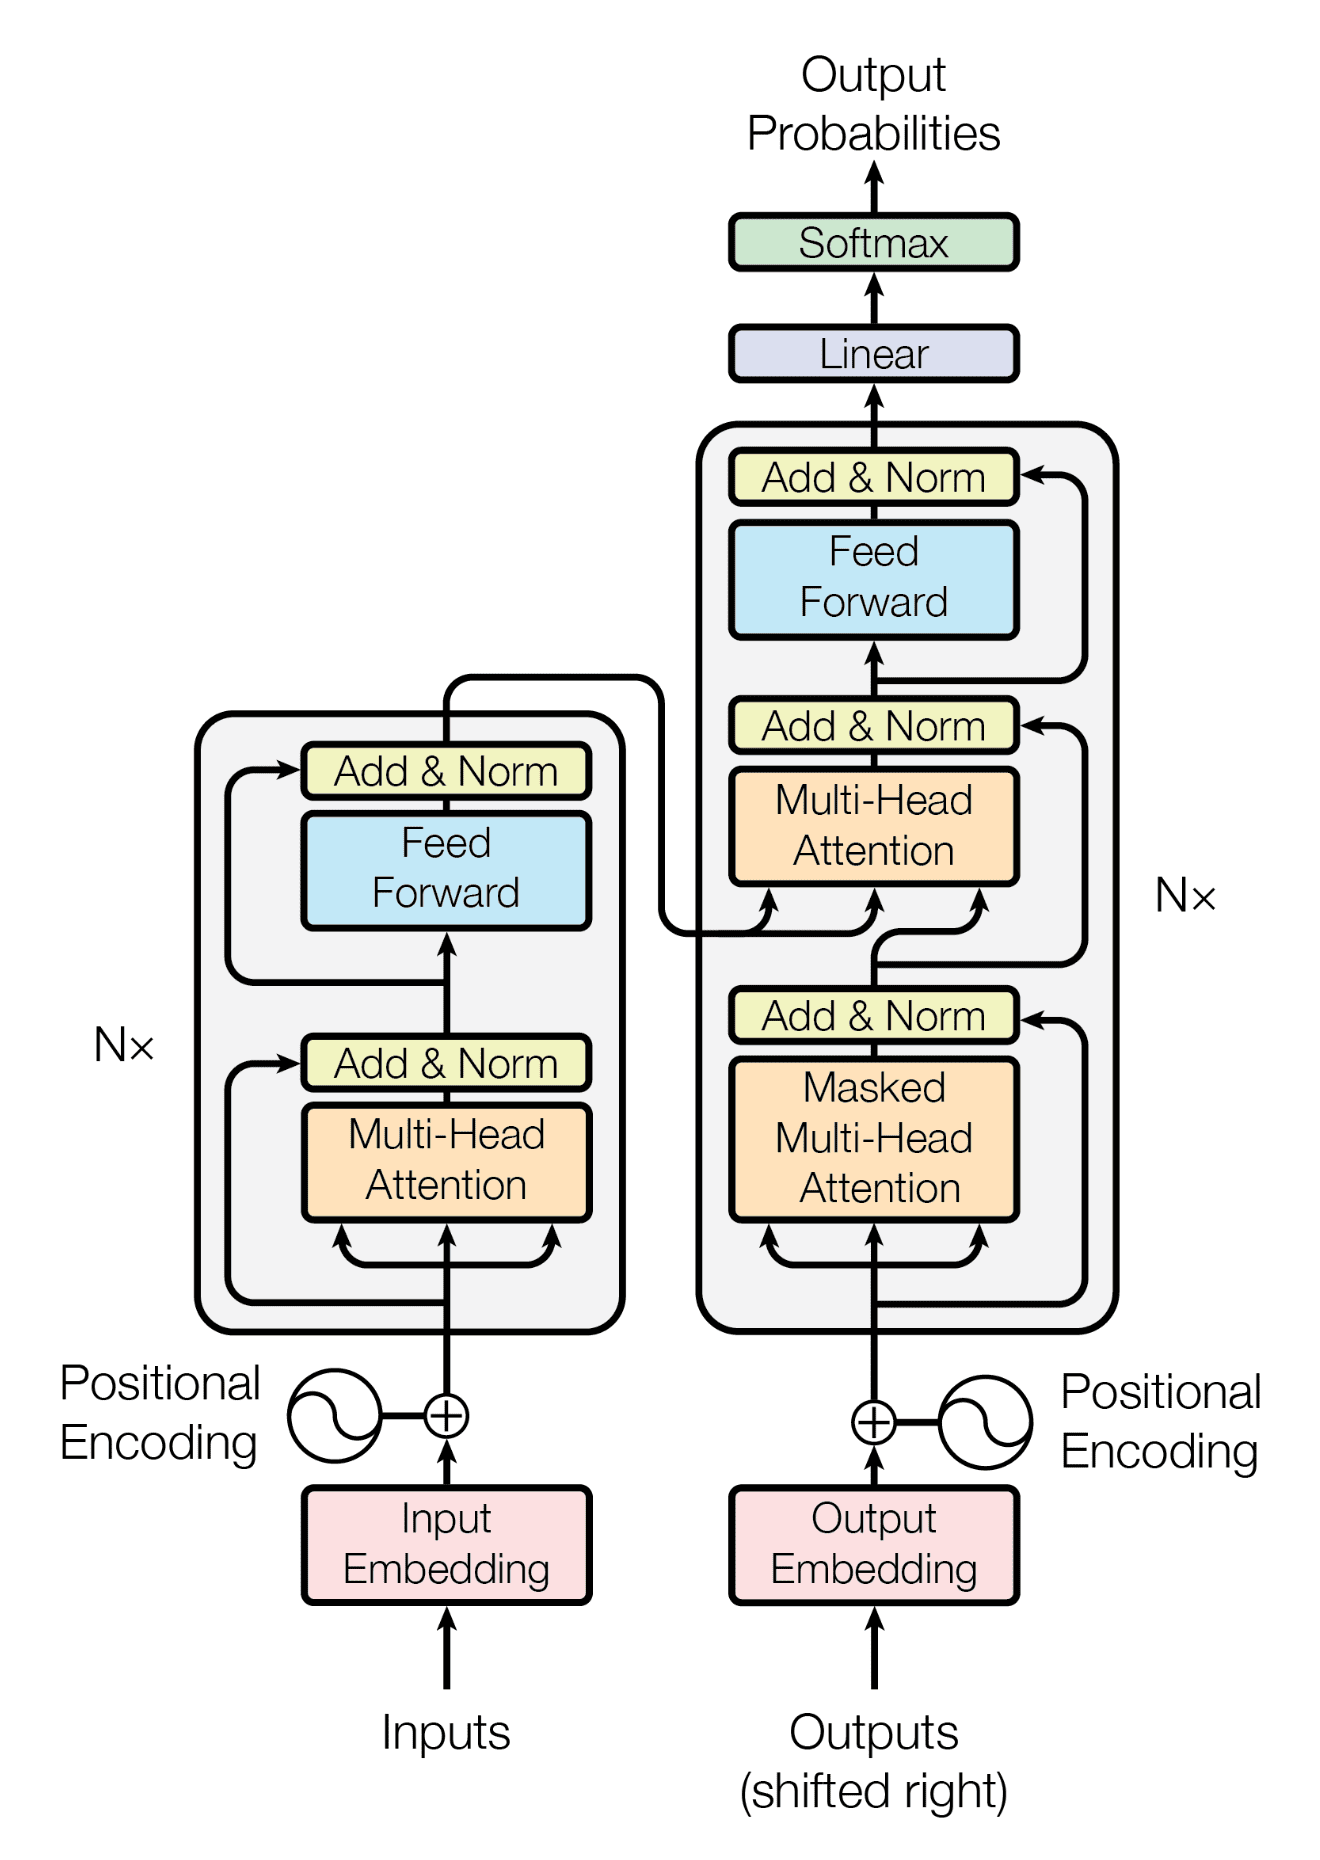
\includegraphics[scale=0.2]{../sections/transformer-architecture/attachments/transformer.png}\caption{The transformer model architecture. The model consists of an encoder (left) and a decoder (right), each containing multiple stacked layers (denoted as N$\times$). The encoder processes input tokens by passing them through embedding layers, positional encoding, multi-head self-attention, and feed-forward networks, with layer normalisation applied after each step. The decoder follows a similar structure but includes an additional masked multi-head attention mechanism to ensure autoregressive generation, preventing positions from attending to future tokens. The final output probabilities are computed through a linear layer and softmax activation.}\label{fig:transformer}\end{figure}

\subsection{Encoder-Decoder Structure}

The encoder transforms an input sequence $\mathbf{X}=(x_1,x_2,\ldots,x_n)$ into a set of continuous representations $\mathbf{H}=(h_1,h_2,\ldots,h_n)$. The decoder then uses $\mathbf{H}$ to generate an output sequence $\mathbf{Y}=(y_1,y_2,\ldots,y_m)$. Each encoder layer is comprised of the following:\begin{enumerate}\item A multi-head self-attention mechanism.\item A position-wise fully connected feed-forward network.\end{enumerate} In the decoder, each layer includes an additional multi-head attention sub-layer that attends over the encoder's output.

\subsection{Self-Attention Mechanism}

The self-attention mechanism allows the model to dynamically focus on different parts of the input sequence. The core operation is the scaled dot-product attention. For given query $\mathbf{Q}$, key $\mathbf{K}$, and value $\mathbf{V}$ matrices, the attention output is computed as \begin{equation}\text{Attention}(\mathbf{Q},\mathbf{K},\mathbf{V})=\text{softmax}\left(\frac{\mathbf{Q}\mathbf{K}^T}{\sqrt{d_k}}\right)\mathbf{V},\end{equation}\label{eq:attention} where $d_k$ is the dimensionality of the key vectors. The factor $\sqrt{d_k}$ helps to maintain stable gradients by scaling down the dot products.

\begin{figure}[htbp]\centering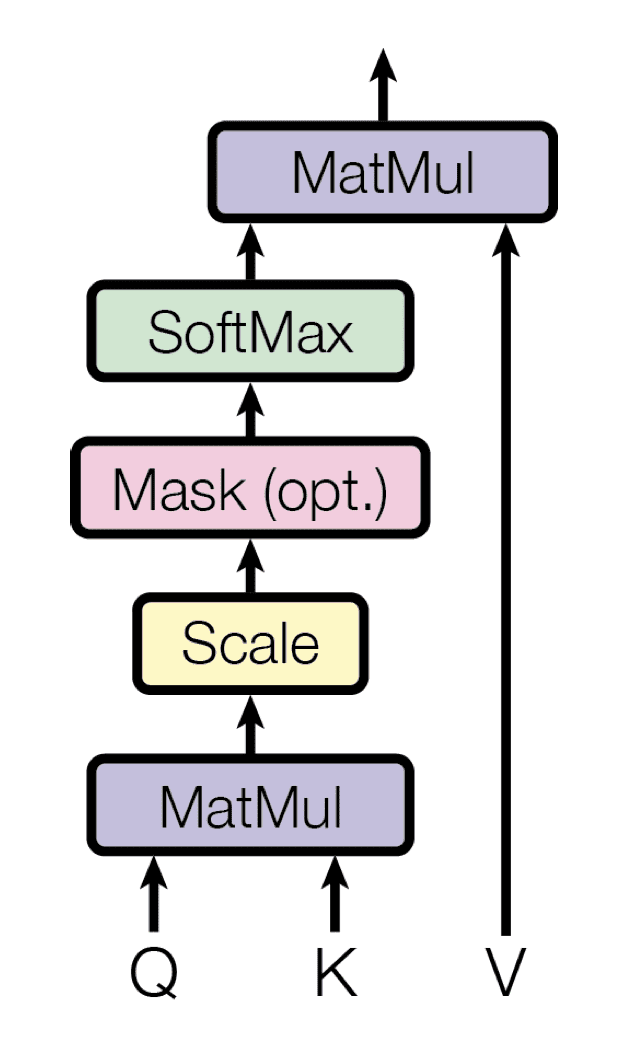
\includegraphics[scale=0.2]{../sections/transformer-architecture/attachments/scaled-dot-product-attention.png}\caption{Illustration of the scaled dot-product attention mechanism. Given query $\mathbf{Q}$, key $\mathbf{K}$, and value $\mathbf{V}$ matrices, the attention scores are computed by performing a matrix multiplication between $\mathbf{Q}$ and $\mathbf{K}^T$, followed by a scaling factor $\frac{1}{\sqrt{d_k}}$ to stabilise gradients. An optional masking step is applied in the decoder to prevent positions from attending to future tokens. The scores are then passed through a softmax function to generate attention weights, which are used to weight the value $\mathbf{V}$ matrix. The final attention output is obtained via matrix multiplication between the attention weights and $\mathbf{V}$, allowing the model to focus on the most relevant parts of the input sequence.}\label{fig:scaled-dot-product-attention}\end{figure}

\subsection{Multi-Head Attention}

To enhance the model's ability to capture various aspects of relationships between tokens, the transformer employs multiple attention heads. This approach involves projecting the queries, keys, and values into different subspaces and computing attention in parallel. It is given by \begin{equation}\text{MultiHead}(\mathbf{Q},\mathbf{K},\mathbf{V})=\text{Concat}(\text{\textbf{head}}_1,\dots,\text{\textbf{head}}_h)\mathbf{W}^O,\end{equation}\label{eq:multihead} where each attention head is given by \begin{equation*}\text{\textbf{head}}_i=\text{Attention}(\mathbf{Q}\mathbf{W}_i^\mathbf{Q},\mathbf{K}\mathbf{W}_i^\mathbf{K},\mathbf{V}\mathbf{W}_i^\mathbf{V}).\end{equation*} Here, $\mathbf{W}_i^\mathbf{Q}$, $\mathbf{W}_i^\mathbf{K}$, $\mathbf{W}_i^\mathbf{V}$, and $\mathbf{W}^\mathbf{O}$ are learned linear projection matrices.

\subsection{Positional Encoding}

Since the transformer does not have any recurrence or convolution to capture sequence order, positional encodings are added to the input embeddings. They inject information about the token positions using sine and cosine functions. The two functions used are \begin{align}\text{PE}_{(pos,2i)}&=\sin\left(\frac{pos}{10000^{\frac{2i}{d_{model}}}}\right),\label{eq:sine-positional-encoding}\\\text{PE}_{(pos,2i+1)}&=\cos\left(\frac{pos}{10000^{\frac{2i}{d_{model}}}}\right).\label{eq:cosine-positional-encoding}\end{align} where $pos$ represents the position in the sequence and $i$ denotes the dimension index. These functions generate unique positional vectors that the model adds to the word embeddings.

\begin{figure}[htbp]\centering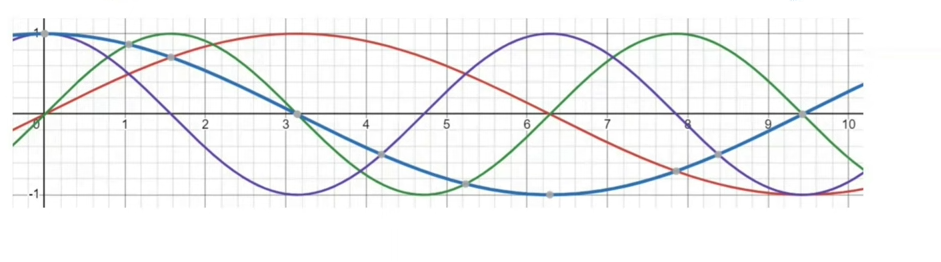
\includegraphics[width=\textwidth]{../sections/transformer-architecture/attachments/positional-encoding.png}\caption{Visualisation of the sine and cosine functions used for positional encoding. Unlike recurrent models, which inherently process sequences step-by-step, transformers lack a built-in notion of order. To overcome this, they use positional encodings, which are added to the input embeddings to provide a unique representation for each position in the sequence. These encodings are generated using sine and cosine functions at different frequencies. The choice of these functions ensure that the encoding captures both absolute and relative positional information. Different frequencies allow the model to recognise repeating patterns and long-range dependencies, even in sequences longer than those seen during training. Since they produce smooth, continuous variations across positions, they provide the model with a structured way to differentiate words based on their position while maintaining meaningful distance relationships between them.}\label{fig:positional-encoding}\end{figure}

\subsection{Feed-Forward Networks}

Each layer in both the encoder and decoder includes a feed-forward network applied to each position independently. This network consists of two linear transformations with a ReLU activation in between. It is given by \begin{equation}\text{FFN}(x)=\max(0,x\mathbf{W}_1+b_1)\mathbf{W}_2+b_2.\end{equation}\label{eq:feed-forward} This component processes the output of the attention mechanisms and adds non-linearity to the model, aiding in the transformation of the attended information.

\section{Experimental Setup and Results}

\subsection{Datasets and Evaluation Metrics}

The transformer model was evaluated on two WMT 2014 translation tasks: English-to-German (4.5 million sentence pairs with a 37,000 token vocabulary using byte-pair encoding) and English-to-French (36 million sentence pairs with a 32,000 token vocabulary). Performance was measured using the BLEU metric, with validation on newstest2013 and testing on newstest2014.

\subsection{Training Details}

The base model used $d_\text{model}=512$, eight attention heads, and inner feedforward dimensionality $d_{ff}=2048$, while the larger model used $d_\text{model}=1024$, 16 heads, and $d_{ff}=4096$. Training employed the Adam optimiser, using hyperparameters $\beta_1=0.9$, $\beta_2=0.98$, and $\epsilon=10^{-9}$, with a custom learning rate schedule:
\begin{equation}
  lrate=d_\text{model}^{-0.5}\cdot\min(step\_num^{-0.5},step\_num \cdot warmup\_steps^{-1.5}).
\end{equation}\label{eq:lrate}
This schedule increased the learning rate linearly during a 4,000-step warmup phase, then decreased it proportionally to the inverse square root of the step number. Regularisation included residual dropout, label smoothing, and beam search decoding. Training was conducted on eight NVIDIA P100 GPUs.

\subsection{Results Analysis}

The transformer demonstrated superior performance, with the base model achieving 27.3 BLEU on English-to-German and 38.1 BLEU on English-to-French, while the large model reached 28.4 and 41.0 BLEU, respectively. These results surpassed all previous single models and even ensembles, with significantly reduced training time. The base model required only about 12 hours of training for the English-to-German task.

Ablation studies confirmed the importance of key architectural decisions: reducing attention heads or layer count decreased performance; replacing dot-product attention with additive attention slowed convergence; removing the scaling factor in attention calculations destabilised training; and positional encodings proved more effective than learned positional embeddings in most scenarios.

\section{Discussion}

The transformer model represents a significant paradigm shift in sequence modelling, addressing fundamental limitations of previous architectures by completely replacing recurrence and convolutions with self-attention mechanisms.

Its key advantage is parallelisability. Unlike RNNs that process tokens sequentially, the transformer's self-attention mechanism attends to all positions simultaneously, substantially reducing training time and improving scalability for large datasets. The multi-head attention mechanism enhances this capability by allowing the model to jointly attend to information from different representation subspaces, capturing various aspects from local syntactic patterns to global semantic relationships.

However, the transformer has limitations. Its computational complexity scales quadratically with sequence length, potentially creating inefficiencies for very long sequences as each token must attend to all others. Future research might explore sparse attention patterns or optimisations to address this constraint. Additionally, while effective, the fixed sinusoidal positional encodings might limit flexibility in representing sequential patterns compared to learned embeddings, though experiments showed comparable results with both approaches.

Despite these considerations, the transformer's impact on NLP is profound. Its strong performance with minimal task-specific modifications suggests that attention-based architectures are broadly applicable across diverse NLP tasks. This aligns with the trend toward more general, transferable models in machine learning, moving away from task-specific architectures toward flexible frameworks that can excel across multiple domains.

\section{Conclusion}

The transformer architecture introduced in \textit{Attention Is All You Need} represents a groundbreaking advancement in sequence modelling that has fundamentally altered NLP research. By demonstrating that a pure attention-based architecture can outperform traditional recurrent and convolutional models, the authors challenged long-held assumptions about sequence processing.

The key innovations - multi-head self-attention, positional encodings, and the encoder-decoder architecture - create a model that effectively captures both local and global dependencies while enabling highly parallel computation. The experimental results validate this approach, with the transformer achieving state-of-the-art BLEU scores on challenging translation benchmarks while requiring significantly less training time than competing models.

Perhaps most significantly, the transformer has proven remarkably adaptable and scalable, serving as the foundation for numerous subsequent innovations in NLP.


\bibliographystyle{plainnat}
\bibliography{../references}

\end{document}
